\subsection{Twitter Dataset}
 For our Twitter dataset, we collected the Tweets of a set of users that tweeted conspiracy theory, misinformation, or authentic news websites from their profile. Utilizing our set of conspiracy theory, misinformation, and authentic news websites and the Python \texttt{Tweepy} we collected the usernames of profiles that tweeted these domains throughout December 2021, totaling 181K different Twitter users. For each of these users, utilizing the \texttt{Tweepy} API we then collected each of their most recent 3240 tweets. Altogether this totaled 446,439,819 different tweets.
 
 In addition, to this core dataset, in order to understand the larger Twitter ecosystem and the relative toxicity and the amounts of misinformation on the platform, we also we utilize the Twitter Streaming API. The Twitter Streaming API gives real-time access to 1\% of public tweets. We continuously collected these tweets between July 10 and and December 21, 2020. We utilize this dataset to understand the characteristics of users within the US-focused and highly politically engaged English-language Twitter ecosystem as a whole. 
 
 
 
 \begin{figure}
    \centering

\begin{tikzpicture}[very thick]
    % Right square
    \node[fill=gray!20,draw=red, minimum size=2cm, inner sep=0pt] (as) {$1.08\%$};
    \node[draw=black,minimum size=2cm, inner sep=0pt, above=-\pgflinewidth of as] (abh) {$0.94\%$};
    \node[draw=black,minimum size=2cm, inner sep=0pt, right=-\pgflinewidth of as] (abv) {$0.87\%$};
    \node[fill=gray!20,draw=blue, minimum size=2cm, inner sep=0pt,  above right=-\pgflinewidth and -\pgflinewidth of as]  {$1.24\%$};
    
    % Side labels
    \node[anchor=east,rotate=90,yshift=0.3cm,xshift=1.0cm] at (as.west) {Conservative};
    \node[anchor=north,] at (as.south) {Liberal};
    \node[anchor=east,rotate=90,yshift=0.3cm,xshift=0.6cm] at (abh.west) {Liberal};
    \node[anchor=north] at (abv.south) {Conservative};
    
    
    % Square label
    \node[xshift=1cm, below=0.7cm of as] {Target};
    
    \node[yshift=1.50cm,xshift=-0.75cm,rotate=90,left=0.5cm of as] {Author};

\end{tikzpicture}
  \caption{Percentage of interactions that are toxic/uncivil in misinformation submissions}
    \label{fig:my_label}
    
\end{figure}    

\begin{figure}
    \centering

\begin{tikzpicture}[very thick]
    % Right square
    \node[fill=gray!20,draw=red, minimum size=2cm, inner sep=0pt] (as) {$0.78\%$};
    \node[draw=black,minimum size=2cm, inner sep=0pt, above=-\pgflinewidth of as] (abh) {$0.83\%$};
    \node[draw=black,minimum size=2cm, inner sep=0pt, right=-\pgflinewidth of as] (abv) {$0.82\%$};
    \node[fill=gray!20,draw=blue, minimum size=2cm, inner sep=0pt,  above right=-\pgflinewidth and -\pgflinewidth of as]  {$0.76\%$};
    
    % Side labels
    \node[anchor=east,rotate=90,yshift=0.3cm,xshift=1.0cm] at (as.west) {Conservative};
    \node[anchor=north,] at (as.south) {Liberal};
    \node[anchor=east,rotate=90,yshift=0.3cm,xshift=0.6cm] at (abh.west) {Liberal};
    \node[anchor=north] at (abv.south) {Conservative};
    
    
    % Square label
    \node[xshift=1cm, below=0.7cm of as] {Target};
    
    \node[yshift=1.50cm,xshift=-0.75cm,rotate=90,left=0.5cm of as] {Author};

\end{tikzpicture}
  \caption{Percentage of interactions that are toxic/uncivil in mainstream submission}
    \label{fig:my_label}
    
\end{figure}   

\begin{table}[b]
\centering
\begin{tabular}{ll}
\toprule
   \multicolumn{2}{c}{\large Toxic Interactions}          \\
   \toprule
      \midrule
      Intercept              & -8.545 ***  &-8.530*** \\               
      \midrule
      User Polarization               & -0.292 & -0.464 \\
      \midrule
      User Polarization Differences    & -2.040*** &-0.782 *** \\
    \midrule
       User Toxicity &   10.557*** &  12.396***\\
      \midrule
       Reciprocity &   3.0863*** &  4.568***\\
      \midrule
\bottomrule
& $\ast p<0.05; ** p<0.01; *** p<0.001$ \\
\end{tabular}
\caption{Caption\label{time}}
\end{table}



\begin{figure}
\begin{minipage}[l]{0.3\textwidth}
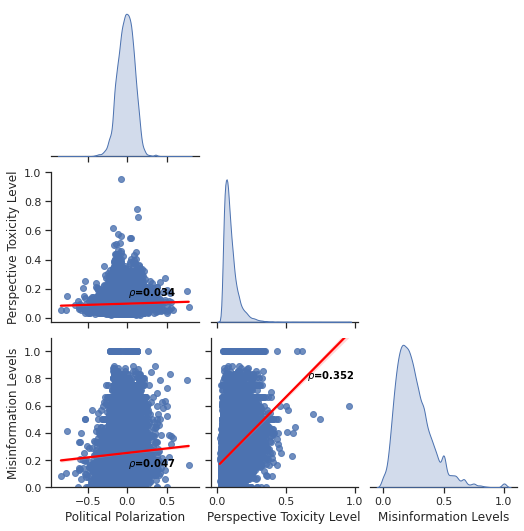
\includegraphics[width=1\columnwidth]{figures/subreddit_distribution.png} 
\end{minipage}
\begin{minipage}[l]{0.3\textwidth}
\caption{\textbf{Misinformation, Toxicity, and Political Polarization Interactions}--- As subreddits increase in misinformation levels, they become more toxic. There is not a large correlation between misinformation levels and the political polarization of subreddits.}
\end{minipage}
\label{figure:subreddit_interaction}
\end{figure}


\begin{table}[b]
\centering
\begin{tabular}{lll}
\toprule
   \multicolumn{3}{c}{\large Number of Comments on Misinfo Submissions}          \\
   \toprule
                                  & {Zero Inflated}  & {Negative Binomial }  \\
                      &       \footnotesize{negative coefficient = } &  \footnotesize{positive coefficient = }\\
                      &       \footnotesize{more likely to get comments} &  \footnotesize{more comments}\\
      \midrule
      Intercept              & 5.810*** & 3.290***  \\               
      \midrule
      Absolute User Polarization               & -7.515***  & -3.550***  \\
      \midrule
      Absolute Subreddit Polarization              & 2.700*** &-0.568* \\
    \midrule
       Subreddit Toxicity & -6.395***   & 5.525*** \\
      \midrule
       User Toxicity &   -13.470*** &  -11.750***\\
      \midrule
      Average Subreddit Comments &  -9.112*** & 1.300***  \\
\bottomrule
& $^\ast p<0.05; \;  ^{**} p<0.01; \; ^{***}p<0.001$ \\

\end{tabular}
\end{table}


\begin{table}[b]
\centering
\begin{tabular}{lll}
\toprule
   \multicolumn{3}{c}{\large Number of Comments on Mainstream Submissions}          \\
   \toprule
                            & {Zero Inflated}  & {Negative Binomial }  \\
                      &       \footnotesize{negative coefficient = } &  \footnotesize{positive coefficient = }\\
                      &       \footnotesize{more likely to get comments} &  \footnotesize{more comments}\\
      \midrule
      Intercept              & 3.054***  &2.436*** \\               
      \midrule
     Absolute User Polarization               & -4.463***  & -2.566***  \\
      \midrule
      Absolute Subreddit Polarization              & 4.296*** &0.415 *** \\
    \midrule
      Subreddit Toxicity & 5.298***  & 12.033*** \\
      \midrule
       User Toxicity &   -12.261*** &  -7.558***\\
      \midrule
      Average Subreddit Comments &  -7.712*** & 0.861***  \\
\bottomrule
& $^\ast p<0.05; \;  ^{**} p<0.01; \; ^{***}p<0.001$ \\
\end{tabular}
\end{table}

\begin{table}[t]
\centering
\small
\begin{tabular}{lrrr}
\toprule
   SEVERE\_TOXICITY \\
   Threshold &   Precision &  Recall  &    F1-Score  \\ \midrule
      0.1  &0.307& 0.576 & 0.400\\
      0.2 &0.414 & 0.390 &0.401 \\
      0.3& 0.484 & 0.295 & 0.367 \\
      0.4 & 0.619 &  0.130 & 0.215 \\
      0.5 & 0.759 & 0.037 & 0.070\\
      0.6 & 0.774 & 0.010 &0.020\\
      0.7 & --- & --- & ---\\
      0.8 & --- & --- &---\\
      0.9 & --- &----& ----\\
\end{tabular}
\caption{Precision, Recall, and F-1 Scores of Perspective API's TOXICITY and SEVERE TOXICITY classifier in correctly labeling social media comments from Deepak et al.~\cite{kumar2021designing}'s dataset as toxic. }
\label{tbl:ergm}
\end{table}

\begin{tabular}{lrrr}
\toprule
TOXICITY \\
    Threshold &   Precision &  Recall  &    F1-Score  \\         \midrule
      0.1  &0.136& 0.991 & 0.240\\
      0.2 &0.152 & 0.975 &0.263 \\
      0.3&0.168 & 0.944 & 0.285 \\
      0.4 & 0.193&  0.841 & 0.314 \\
      0.5 & 0.222 & 0.692 & 0.337\\
      0.6 & 0.254 & 0.533 &0.344\\
      0.7 & 0.308 & 0.345 & 0.325\\
      0.8 & 0.402 & 0.185 &0.254\\
      0.9 & 0.594 &0.075& 0.133\\
      
\end{tabular}

\begin{figure}
\begin{minipage}[l]{0.8\textwidth}
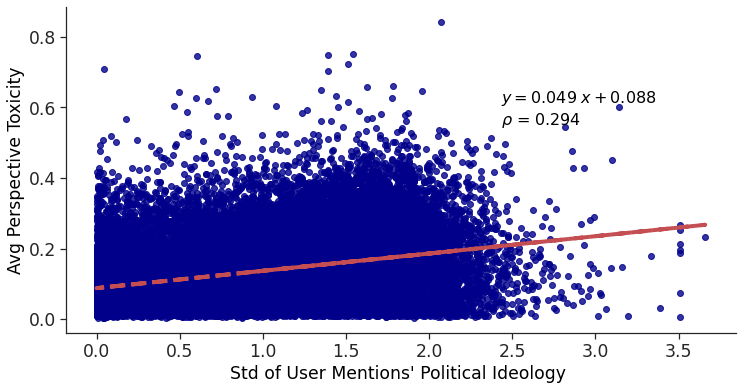
\includegraphics[width=1\columnwidth]{figures/std_user_mentions.png} 
\end{minipage}

\begin{minipage}[l]{1\textwidth}
\caption{Users in the political center have the highest \textbf{average toxicity} compared to users on the political ends.   \label{fig:toxicity-vs-polarization}}
\end{minipage}

\end{figure}
%Finally, to ensure that we properly capture the behavior of those that twee mainstream and misinformation on Twitter, we gathered 16,000 different accounts that tweeted mainstream/authentic news domains between September 5, 2022, and November 2, 2022, as well as another 18,000  accounts that tweeted a misinformation domain link between  September 5, 2022, and November 2, 2022,  as well.

\begin{table}[t]
\centering
\small
\begin{minipage}[l]{0.4\textwidth}
\begin{tabular}{lrrr}
\toprule
   SEVERE\_TOXICITY \\
   Threshold &   Precision   \\ \midrule
      0.1  &0.307\\
      0.2 &0.414  \\
      0.3& 0.484  \\
      0.4 & 0.619\\
      0.5 & 0.759\\
      0.6 & 0.774 \\
      0.7 & --- & \\
      0.8 & --- & \\
      0.9 & --- &\
\end{tabular}
\end{minipage}
\begin{minipage}[l]{0.4\textwidth}
\caption{Precision Peerspective API's TOXICITY and SEVERE TOXICITY classifier in correctly labeling social media comments from Deepak et al.~\cite{kumar2021designing}'s dataset as toxic. }
\end{minipage}
\label{tbl:ergm}
\end{table}


\begin{table*}
\centering
\scriptsize
%\fontsize{8.5pt}{10pt}
\selectfont
\setlength{\tabcolsep}{4pt}
\begin{tabularx}{\textwidth}{l|llrXr}
\toprule
Topic &  {Keywords} & \# Tweets &  \# Toxic Tweets & Example Tweet  & Approx. Part. & Approx. Part. of Toxic\\ \midrule


 3 & putin,russia,ukraine,war,civilian  &1850209 & 18421  & RUSSIA FAILED. UKRAINE WON! Russia is destined to FAIL under maniacal Putin. It is a pariah among the world amp; its inhumane cruelty has been exposed: murdering civilians, raping women amp; children. What a collection of barbarians. Enemy of humanity. & -0.273 \\ %\hline



 1& republican, gop, demcorat, party,maga & 32,675 & Republicans are just disgusting, lying, no good, power grabbing, coward bastards! & -0.191 \\


  2 & block, fascist, asshole, bigot, post & 25,751 & @LieuColumbo @mattybones8 @realDailyWire @joerogan @jordanbpeterson Leave you alone? You really are a miserable person, aren’t you? I have tried to be nice. But, honestly? Go fuck yourself, buddy. We’re fucking through here & -0.112\\



  4 & nazi, hitler, jew, fascist, antisemite & 13,765 & Nazi punks fuc off!!! & -0.144 \\

  5 & racist, black, white, supremracist, color & 11,773 &  Hes a racist pig & -0.058 \\
 6 & dickhead, lol,bitf*cked, margin, f*ck & 10,873 &   Who is that asshole? & -0.017 \\

 7 & abort, baby, brith, unborn,proliferate & 10,272 & Until those little creatures can take the "breath" of life on their own, then it is up to WOMEN to decide what is to be done! Fuck you and you notions of patriarchal control of women\'s bodies. Until further notice we ARE the God in your life! & 0.146 \\

  8 & phedophilia, pedo, child, graphic,pervert & 9,130 &Ladies and Gentlemen the PedoDent of the United States $\#$PedoHitler & 0.235   \\

  9 & nigga, rap, aint, song, yo & 8,392 & I was so mad but I had to be cool. Cause bitches is really out here setting niggas up. And when you gotta street nigga, they gotta protect themselves all the time. & -0.066 \\


  10 & twitter, tweet,elon, retweet, musk & 7,284 &Twitter isnt a representative democracy and we dont give criminals and sociopaths representation when we are enjoying one. Which you already know, you disingenuous fuck. & -0.085 \\

\bottomrule
\end{tabularx}
\caption{\label{tab:narratives} Top toxic topics---by number of tweets---in our dataset.} %\todo{how was this selection made? Sounds vague.
\end{table*}


\begin{table*}
\centering
\scriptsize
%\fontsize{8.5pt}{10pt}
\selectfont
\setlength{\tabcolsep}{4pt}
\begin{tabularx}{\textwidth}{l|lrXr}
\toprule
Topic &  {Keywords} & \# Toxic Tweets & Example Tweet  & Approx. Partisanship\\ \midrule
 1& spy, china, bang, community,fang & 142 &You fucked a Chinese Communist Party spy.  You should probably just shut up, Corky.  & 1.000 \\
\bottomrule
\end{tabularx}
\caption{\label{tab:narratives} Top toxic topics  with at least 100 tweets and 10 users---by conservative tilt---in our dataset.} %\todo{how was this selection made? Sounds vague.
\end{table*}


\begin{table*}
\centering
\scriptsize
%\fontsize{8.5pt}{10pt}
\selectfont
\setlength{\tabcolsep}{4pt}
\begin{tabularx}{\textwidth}{l|lrXr}
\toprule
Topic &  {Keywords} & \# Toxic Tweets & Example Tweet  & Approx. Partisanship\\ \midrule
 1& spy, china, bang, community,fang & 142 &You fucked a Chinese Communist Party spy.  You should probably just shut up, Corky.  & 1.000 \\
2 & break, liar, idiot, scumbag,alert &268 &   @Breaking911 Piece of shit & 0.849 \\
3  & phedophile, chief, burn, dead, asshole &154 &  @ProudElephantUS Sl* u *t & 0.823 \\

4  & biden, joe, hell, hunter, die &213 & @BidensWins Fuck u Biden & 0.780\\
5 & rino, piece, rishi,sunak,worthless &236 & Fucking rino mother fucker!!!! & 0.778 \\
6  & fuck, hag, diseased, crazy, liberal &271  &@GioBruno1600 Piece of Shit!!' & 0.774 \\

7 & china, jihad, butt, biden, kiss & 140 & CHINA'S QUID PRO QUO JIHAD BUTT KISS PUPPET, BULLSHIT ARTIST JOE BIDEN...COMPLETE WITH DEMENTIA!!!& 0.767 \\

8  & schiff, schumer, adam,chuck, lie & 279 & @RepAdamSchiff Schiff is a lying evil scumbag!  & 0.758 \\
9  & baby, kill, womb,birth, unborn & 257 & URGENT: YOU CAN STILL KILL YOUR BABIES  & 0.750 \\
10  & jackson, ketanji, child, brown, porn & 108 & Kiddie Porn and Child Molester Problems the Big issue with Judge Ketanji Brown Jackson - Children Raped and Sodomized & 0.728 \\
\bottomrule
\end{tabularx}
\caption{\label{tab:narratives} Top toxic topics  with at least 100 tweets and 10 users---by conservative tilt---in our dataset.} %\todo{how was this selection made? Sounds vague.
\end{table*}


\begin{table*}
\centering
\scriptsize
%\fontsize{8.5pt}{10pt}
\selectfont
\setlength{\tabcolsep}{4pt}
\begin{tabularx}{\textwidth}{l|lrXr}
\toprule
Topic &  {Keywords} & \# Toxic Tweets & Example Tweet  & Approx. Partisanship\\ \midrule
 1& mr, rott, fuck, motherfuck,treason & 155 &@BaddCompani Fcuk that guy  & -1.15\\
 2& gay, death, facist, homophobe,asswipe & 201 &$\#$DeathSantis the Fascist& -1.13 \\
  3& white, racist, her, stupid,damn & 191 &@notcapnamerica She sounds like a whole ass idiot. He has killed children. Fuck him and her.& -1.03 \\

  4 & lie, fuck, guy, piece,idiot & 530 &@Acyn You. You fucking Nazi!& -1.00\\

  5 & gqp, nazi, party, homophobe,vote & 215 &@RBraceySherman 3/what pisses me off the most about bs like UR whiny privileged article is that Trump ; GQP did so much fucking damage…U all expect 1 election (an election where many failed 2vote in Dem at local level)…U expect a quick fix?! Stop whining ,attack GQP not Dems;fucking vote. !& -0.921\\

  6 & elise,bottom,feed,cheat,filthy & 342 &@EliseStefanik @seanhannity Batshit crazy @elisestafanik please just go crawl back under your porch and stay there.& -0.917\\
   7 & whore,hooker,dick,trash,douchebag & 342 &  @MysterySolvent Asswipe& -0.911\\

   8 & putin,ukraine,slava,thug,war & 131 & @olex\_scherba $\#$RussiaIsATerroristState& --0.907\\

   9 & marg,cult,guilty,violation,beat & 119 & @RepMTG You're so full of shit, Marge.& --0.883\\

   10 & cathowrn, cousin,madison, orgy, nazi &287 & @CawthornforNC fuck you, asswipe.  & -0.872 \\
\bottomrule
\end{tabularx}
\caption{\label{tab:narratives} Top toxic topics  with at least 100 tweets and 10 users---by liberal tilt---in our dataset.} %\todo{how was this selection made? Sounds vague.
\end{table*}


\begin{figure}
\begin{minipage}[l]{0.48\textwidth}
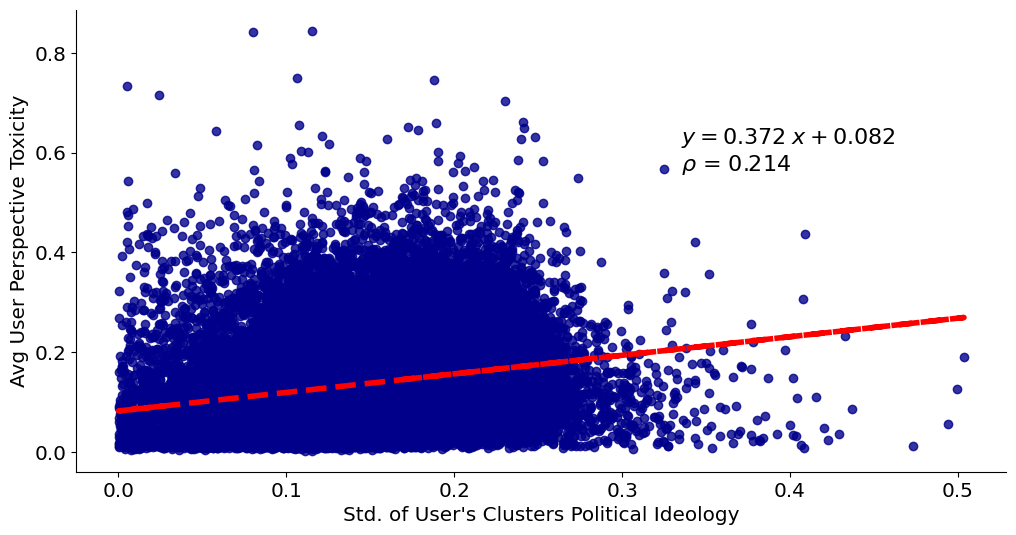
\includegraphics[width=1\columnwidth]{figures/toxicity_vs_cluster_std.png} 
\end{minipage}
\begin{minipage}[l]{0.48\textwidth}
\caption{As previously also found in our analysis of user characteristics (Section~\ref{sec:calculated}), we find that as users engage in a wider window of topics of particular political ideologies, the more toxic their tweeted content\label{fig:toxicity-vs-var}}
\end{minipage}

\end{figure}

% \subsection{Misinformation and Authentic News Dataset}

%To understand how users who utilize questionable sources on Twitter interact with other users, we first curate a list of websites that often publish unreliable and otherwise unverifiable information. As a control, we further gather a separate list of websites that publish reliable and verifiable information.  Specifically, we aggregate together unreliable and reliable news domains previously gathered by Iffy News,\footnote{\url{https://iffy.news/index}} OpenSources,\footnote{\url{https://github.com/several27/FakeNewsCorpus}} Politifact,\footnote{\url{https://www.politifact.com/article/2017/apr/20/politifacts-guide-fake-news-websites-and-what-they/}} Snopes,\footnote{\url{https://github.com/Aloisius/fake-news}} and Melissa Zimdars\footnote{\url{https://library.athenstech.edu/fake}}, Hanley et~al.~\cite{hanley2022golden}, and MediaBias/FactCheck. We note for MediaBias/FactCheck that we father our set of  unreliable news domains from the set of websites labeled as ``questionable sources''; similarly we gathered our set of reliable websites from those labeled as center-right, center-left, and center. Altogether, we collect a total of 1,376 unreliable news domains and 2,285 reliable news websites. Our list of misinformation domains included websites such as globalresearch.ca, infowars, and thegatewaypundit.com which have been documented as being parts of toxic political echo-chambers~\cite{starbird2018ecosystem}. Our list of reliable news domains consists of websites across the political including foxnews.com, dailywire.com, nytimes.com, and cnn.com.




 %Lastly, we note that. %Altogether we gather

% In addition to this core dataset, we also utilize the Twitter Streaming API to understand the larger Twitter ecosystem and the relative toxicity and amounts of misinformation on the platform. The Twitter Streaming API gives real-time access to 1\% of public tweets. We continuously collected these tweets between July 10 and December 21, 2022. We utilize this dataset to understand the characteristics of English-language Twitter. 






%As found by Kumar~\textit{et al.}~\cite{kumar2021designing}, utilizing this particular classifier at a threshold of 0.6~\cite{kumar2021designing}, provides an acceptable precision for identifying toxic online content across different subgroups of users. Throughout this work, we thus consider a tweet as toxic if as a SEVERE\_TOXICITY score above 0.6.

\begin{figure}
\begin{minipage}[l]{0.8\textwidth}
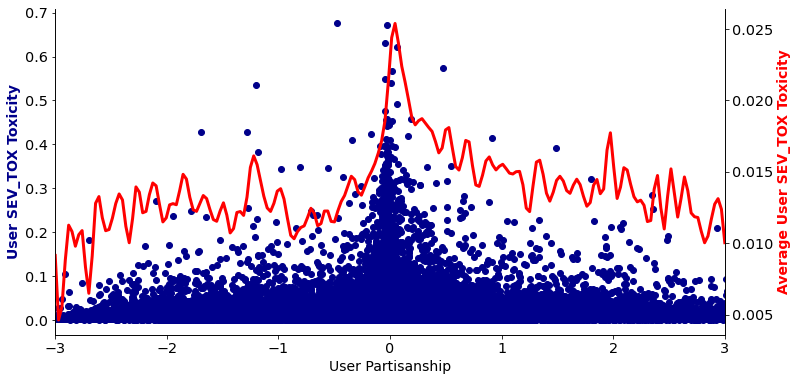
\includegraphics[width=1\columnwidth]{figures/user_toxicity_vs_partisanship.png} 
\end{minipage}

\begin{minipage}[l]{1\textwidth}
\caption{Users in the political center have the highest \textbf{average toxicity} compared to more liberal or conservative users. \label{fig:toxicity-vs-polarization}}
\end{minipage}

\end{figure}


\begin{figure}
    \centering
\begin{minipage}[l]{0.6\textwidth}
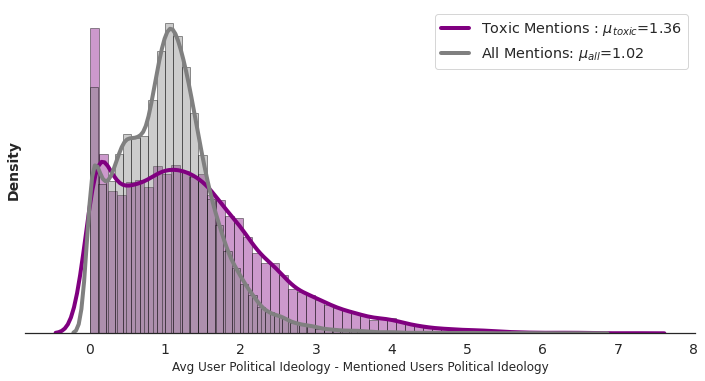
\includegraphics[width=1\columnwidth]{figures/all_vs_toxic_political_mentions.png} 
\end{minipage}
\begin{minipage}[l]{0.33\textwidth}
\caption{ When users mention (@) users that are more politically different than themselves, they are more likely to be toxic. On average Toxic Tweets  (SEVERE\_TOXICITY> 0.3) occur in mentions with more disparate political ideologies compared to all tweet interactions.  \label{fig:politican-diff-toxicity}}
\end{minipage}
\end{figure}



\begin{table}[t]
\centering
\scriptsize
\begin{tabular}{lrrr}
\toprule
   SEVERE\_TOXICITY \\
   Threshold &   Precision &  Recall  &    F1-Score  \\ \midrule
      0.05 & 0.284 & 0.624 & 0.390 \\  
      0.10  &0.307& 0.576 & 0.400\\
      0.15 & 0.321&0.543 & 0.404 \\
      0.20 &0.414 & 0.390 &0.401 \\
      0.25& 0.466 & 0.311& 0.373 \\
      0.30& 0.484 & 0.295 & 0.367 \\
      0.35& 0.530 & 0.246 & 0.336 \\
      0.40 & 0.619 &  0.130 & 0.215 \\
      0.45 & 0.651 &  0.099 & 0.172\\
      0.50 & 0.759 & 0.037 & 0.070\\
      0.55 & 0.766 & 0.015 & 0.029\\
      0.60 & 0.774 & 0.010 &0.020\\
      0.65 & --- & ---  &--- \\
      0.70 & ---  & ---  &--- \\
       0.75 & ---  & ---  &--- \\
       0.80 & ---  & ---  &--- \\
       0.85 & ---  & ---  &--- \\
       0.90 & ---  & ---  &--- \\
\end{tabular}
\begin{tabular}{lrrr}
\toprule
   TOXICITY \\
   Threshold &   Precision &  Recall  &    F1-Score  \\ \midrule
      0.05 & 0.129 & 0.996& 0.228 \\  
      0.10  &0.136& 0.991 & 0.239\\
      0.15 & 0.144&0.984 & 0.251 \\
      0.20 &0.152 & 0.975 &0.263 \\
      0.25& 0.159 & 0.965& 0.272\\
      0.30& 0.168 & 0.944 & 0.285 \\
      0.35& 0.179 & 0.908 & 0.300 \\
      0.40 & 0.193 &  0.841 & 0.314 \\
      0.45 & 0.208 &  0.771 & 0.327\\
      0.50 & 0.222 & 0.693 & 0.336\\
      0.55 & 0.234 & 0.617 & 0.343\\
      0.60 & 0.254 & 0.533 &0.344\\
      0.65 & 0.279 & 0.432 &0.339\\
      0.70 & 0.308 & 0.345 &0.325\\
       0.75 & 0.336 & 0.281 &0.306\\
       0.80 & 0.402 & 0.186 &0.254\\
       0.85 & 0.466 & 0.137 &0.211\\
       0.90 & 0.594 & 0.075 &0.133\\
\end{tabular}
\caption{Precision, Recall, and F-1 Scores of Perspective API's TOXICITY and SEVERE TOXICITY classifier in correctly labeling social media comments from Kumar et~al.~\cite{kumar2021designing}'s dataset as toxic.}
\label{tbl:perspective-f1}
\vspace{-15pt}
\end{table}


\begin{table}
    \small
    \centering
    \begin{tabularx}{0.7\columnwidth}{l|lrr}
    \toprule
  Adjusted R-squared:  0.373  & Coefficient  & Std. Error & Adj. Sum Sq. \\    \midrule
  Intercept &${-0.108}^{***}$& 0.012 & 0.983\\
  Log \# Users & $-0.005$ & 0.003 &0.029 \\
  Percentage Verified & $0.040$& 0.020 & 0.015 \\
  Avg User Toxicity in Cluster & $\textbf{2.897}^{***}$ & 0.065 & \textbf{16.95} \\
 Abs Cluster Political Ideology  & $-0.093^{***}$ & 0.015  & 0.352\\
 Std Cluster Political Ideology  &  $0.0415^{***}$ & 0.010 &0.072	\\
  Left/Right  & 0.0054& 0.003 &0.026\\
    \bottomrule
     \multicolumn{4}{c}{ $^\ast p<0.05; \;  ^{**} p<0.01; \; ^{***}p<0.001$ }
    \end{tabularx}
  \caption{Linear fit on factors in the toxicity in individual topic clusters. } 
   \vspace{-15pt}
   \label{table:regression-cluster-toxicity}
\end{table}

\begin{table*}
\centering
\scriptsize
%\fontsize{8.5pt}{10pt}
\selectfont
\setlength{\tabcolsep}{4pt}
\begin{tabularx}{\textwidth}{l|XrrrXrrr}
\toprule
 &   &  &   \# Toxic  & Avg.& Example & Avg.  & Avg. Partisan  & Partisan \\
 Topic& {Keywords}&\# Tweets & Tweets & Toxicity &  Tweet  & Partisan. & of Toxic Users& Std. \\

\midrule
1 & mastriano, thanmaga, antisemitic, louder, mastribator & 128& 74 (57.82\%) &0.492 & Sen Mastriano You're an anti-Semitic POS.
 & -2.176& -0.682 & 1.791 \\
 2& delta, operator, fking, dawn, nightclub & 284 & 89 (31.34\%)& 0.321 &I Have To Kill This Guy Before He Kills Us:' Army Vet Says After Harrowing Nightclub Shooting & 1.034& 0.152 & 1.693 \\

 3 & defeatist, sore, winning, lose, metabolize, & 476 & 127 (26.68\%) & 0.270&Same hypocrites who say the losers should lose gracefully on the very rare occasion they actually win anything. & -0.586 &-0.152 & 1.548 \\

4 & scalise, saved, steve, trumpshit, sleazy & 246 & 65 (26.42\%)& 0.282 & EWhen bringing up that Steve Scalise was also attacked can we also bring up the fact it was a gay black woman who saved his ass & -0.565 &-0.900& 1.548 \\

5 & tillis, thom, burr, nc, sen, establishment & 2,199&271 (12.32\%)& 0.143 & Sen Thom Tillis Traitor 
You've always been a RINO
NC must be ashamed of you  & 0.049 & 0.372 & 1.424 \\
 
\bottomrule 
\end{tabularx}
\caption{\label{tab:variance-topics} Top toxic topics by variation in user partisanship.} 
\vspace{-10pt}
\end{table*}